% document type
\documentclass[12pt]{article}

\usepackage[a4paper, includefoot,
            left=3cm, right=1cm,
            top=1.5cm, bottom=1.5cm,
            headsep=1cm, footskip=1cm]{geometry}
%Russian-specific packages
%--------------------------------------
\usepackage[T2A]{fontenc}
\usepackage[utf8]{inputenc}
\usepackage[russian]{babel}
%--------------------------------------
 
%Hyphenation rules
%--------------------------------------
\usepackage{hyphenat}
\usepackage{tempora}

% в преамбуле
\usepackage{subcaption}

\usepackage{physics}
\usepackage{fixint}
\usepackage{tikz}
\usepackage{hyperref}
\usepackage{graphicx} % для вставки картинок
\usepackage{amssymb,amsfonts,amsmath,amsthm} % математические дополнения от АМС
\usepackage{indentfirst}
\usepackage{nicefrac,xfrac}
\usepackage{subcaption}

\usepackage{cmap}

\linespread{1.3} % полуторный интервал
\frenchspacing

\newcommand*{\figref}[2][]{\hyperref[#2]{Рис.~\ref*{#2}#1}}
\newcommand*{\tabref}[2][]{\hyperref[#2]{Табл.~\ref*{#2}#1}}
% \newcommand*{\tblref}[1]{\hyperref[#1]{Table~\ref*{#1}}}
\newcommand*{\secref}[1]{\hyperref[#1]{Section~\ref*{#1}}}
% \newcommand*{\secsref}[1]{\hyperref[#1]{Sections~\ref*{#1}}}
% \newcommand*{\introref}[1]{\hyperref[#1]{Introduction}}

\begin{document}
	\begin{titlepage}
    \begin{center}
    % \vspace{-3em}
    {\small\textsc{Нижегородский государственный университет имени Н.\,И. Лобачевского}}
    \vskip 2pt \hrule \vskip 3pt
    {\small\textsc{Высшая школа общей и прикладной физики}}

    \vfill


    {{\large Отчет по лабораторной работе}\vskip 12 pt {\Large \bfseries Низкочастотные процессы в многомодовом твердотельном лазере}}

        
    \vspace{2cm}
    {\large Работу выполнили студенты \\[0.5em]{\Large \bfseries Поляков Андрей, Козлов Александр}}

    \end{center}

    \vfill

    \begin{center}
    {Нижний Новгород, \today}
    \end{center}
\end{titlepage}
	\setcounter{page}{2}

	\tableofcontents
	\newpage

	\section{Основные элементы теории}

	\subsection{Неодимовые лазеры}

	Неодимовые лазеры работают по четырёхуровневой схеме. На \figref{fig:energy_scheme} представлена упрощенная схема энергетических уровней иона $\mathrm{Nd}^{3+}$ в алюмоиттриевом гранате. Эти уровни обусловлены переходами внутри 4f электронной оболчки, которая является внутренней и хорошо экранирована от кристаллического поля, в связи с чем уровни узкие.

	\begin{figure}[htbp]
		\centering
		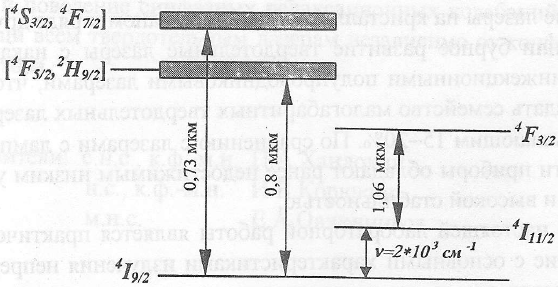
\includegraphics[width=\textwidth]{../figures/energy_scheme}
		\caption{Упрощенная схема энергетических уровней иона $\mathrm{Nd}^{3+}$ в алюмоиттриевом гранате.}
		\label{fig:energy_scheme}
	\end{figure}

	Обычно используется полоса накачки $0.8\,\text{мкм}$, которая связана быстрой ($\sim10^{-7}\,\textnormal{с}$) безызлучательной релаксацией с уровнем ${}^4\mathrm{F}_{3/2}$. Этот уровень метастабилен ($T_1\approx0.23\,\textnormal{мс}$). Среди возможных переходов с уровня ${}^4\mathrm{F}_{3/2}$ на нижележащие наиболее интенсивным является переход ${}^4\mathrm{F}_{3/2} \rightarrow {}^4\mathrm{I}_{11/2}$. Уровень ${}^4\mathrm{I}_{11/2}$ связан с уровнем ${}^4\mathrm{I}_{9/2}$ безызлучательной релаксацией, поэтому его можно считать пустым.

	Выходит, что в кристалле Nd:YAG переход ${}^4\mathrm{F}_{3/2}\rightarrow{}^4\mathrm{I}_{11/2}$ хорошо подходит для получения лазерной генерации по четырёхуровневой схеме. Этот переход имеет длину волны $\lambda=$~$1.064\,\textnormal{мкм}$ и однородно уширен вследствие взаимодействия с фононами решетки. Ему соответствует ширина $\delta\nu = 195\,\textnormal{ГГц}$ при температуре $T=300\,\textnormal{К}$.

	\subsection{Уравнения многомодового лазера}

	Для описания динамических процессов в твердотельных лазерах с резонаторами Фабри-Перо традиционно применяются балансные уравнения. В безразмерном виде для идеализированного одномерного случая они выглядят следующим образом:
	\begin{equation}\label{eq:1}
		\begin{cases}
			\dv{\tau} I_p(\tau) = G I_p(\tau)\qty(\gamma_p \int\limits_0^L\mathcal{N}(z,\tau) \Psi_p^2(z) \dd{z} - 1),\\
			\dv{\tau} \mathcal{N}(z,\tau) = A - \mathcal{N}(z,\tau)\qty(1 + \sum\limits_{p=1}^{M} \gamma_p I_p(\tau)\Psi_p^2(z)).
		\end{cases}
	\end{equation}

	В этой модели подразумевается, что резонатор имеет длину $L$ и полностью заполнен активной средой; $I_p = \abs{E_p}^2$ --- интенсивность поля $p$-ой моды, $p=1,\ldots,M$; $\mathcal{N}$ --- разность населенностей рабочих уровней; $G = T_1 / T_\textnormal{с}$; $\gamma_p$ --- коэффициент усиления $p$-ой моды, нормированный на коэффициент усиления моды, ближайшей к центру линии усиления ($\gamma_p\le1$); $A$ --- параметр накачки; $\Psi_p(z) = \sqrt{2}\sin (\pi q_p z / L)$ --- собственная функция холодного резонатора; $q_p$ --- (большое целое) число полуволн, укладывающихся в длине $L$; $\tau = t/T_1$ --- безразмерное время.

	Уравнение \ref{eq:1} можно упростить, если разложить разность населенностей $N(z,\tau)$ в пространственный ряд Фурье и отбросить все гармоники, кроме тех, которые непосредственно входят в уравнения для интенсивности мод. Тогда получаем:
	\begin{equation}\label{eq:2}
		\begin{cases}
			\dv{\tau} I_p = G I_p \qty[\gamma_p \qty(N_0 - N_p) - 1],\\
			\dv{\tau} N_0 = A - \qty(1 + \sum\limits_{p=1}^{M} \gamma_p I_p(\tau))N_0 + \sum\limits_{p=1}^{M} \gamma_p I_p(\tau) N_p,\\
			\dv{\tau} N_p = - (1 + \sum\limits_{p=1}^{M} \gamma_p I_p(\tau))N_p + \frac12 \gamma_p I_p(\tau) N_0.			
		\end{cases}
	\end{equation}
	Здесь пространственно однородная компонента
	\begin{equation}
		N_0 = \frac1L \int\limits_0^L \mathcal{N}(z) \dd{z}
	\end{equation}
	и $p$-ая гармоника инверсии
	\begin{equation}\label{eq:N_p}
		N_p = \frac1L \int\limits_0^L \mathcal{N}(z) \cos (\pi q_p z/L)\dd{z}.
	\end{equation}

	\subsection{Стационарная генерация}

	Система \ref{eq:2} имеет два стационарных решения. Первое соответствует отсутствию генерации 
	\begin{equation}
		\overline{I}_p = 0,\quad \overline{N}_p = 0,\quad \overline{N}_0 = A.
	\end{equation}
	Оно устойчиво при $A\le1$ и неустойчиво при
	\begin{equation}\label{eq:samovozb}
		A > 1.
	\end{equation}
	Это так называемое условие самовозбуждения лазера.

	Второе стационарное решение соответствует многомодовой лазерной генерации:
	\begin{equation}\label{eq:2nd_stac}
		\begin{split}
			&\overline{N}_p = \overline{N}_0 - 1/\gamma_p,\quad \overline{I}_p =\qty(\overline{N}_p - 1/\gamma_p)/\gamma_p\qty[S_1 - (M-1/2)\overline{N}_0],\\
			&\overline{N}_0 = \dfrac{2S_1 + A\qty(M-1/2) - \sqrt{\qty[2S_1 + A\qty(M-1/2)]^2 - 4\qty(M-1/2)(AS_1 + S_2)}}{2M-1},\\
			&S_1 = \sum\limits_{p=1}^{M} 1/\gamma_p,\quad S_2 = \sum\limits_{p=1}^{M}\qty(1/\gamma_p)^2.
		\end{split}
	\end{equation}
	Оказывается, что при выполнении условия самовозбуждения (\ref{eq:samovozb}) второе стационарное решение всегда устойчиво. Таким образом, при повышении мощности накачки порогового значения в твердотельном лазере развивается многомодовая генерация. Число генерируемых мод зависит от уровня накачки $A$ и параметров линии усиления.

	\subsection{Спектр релаксационных колебаний}

	Проведём линейный анализ устойчивости второго стационарного решения (\ref{eq:2nd_stac}). Аналитически это можно сделать лишь в двух случаях: одномодовый случай и случай равного усиления мод.

	Рассмотрим сперва одномодовый режим. В этом случае мы можем исключить $N_1$ (пренебрегаем эффектом выжигания дырок), тогда 
	\begin{equation}\label{eq:one_mode}
		\begin{cases}
			\dv{\tau} I = G I \qty(N_0 - N_p),\\
			\dv{\tau} N_0 = A - \qty(1 + I)N_0.			
		\end{cases}
	\end{equation}
	Нетривиальное стационарное состояние
	\begin{equation}\label{eq:sost_ravn}
		\overline{I} = A-1,\quad \overline{N}_0 = 1
	\end{equation}
	имеет физический смысл лишь при $A>1$. Линеаризация системы \ref{eq:one_mode} в окрестности состояния равновесия (\ref{eq:sost_ravn}) достигается заменой переменных $I = \overline{I} + \xi,\; N_0 = \overline{N}_0 + \eta$, и приводит к системе
	\begin{equation}\label{eq:lin_eq}
		\begin{cases}
			\dv{\tau} \xi = G \eta \qty(N_0 - N_p),\\
			\dv{\tau} \eta = -A\eta-\xi.			
		\end{cases}
	\end{equation}
	Что приводит к характеристическому уравнению
	\begin{equation}
		\lambda^2 + A\lambda + G\qty(A-1)=0,
	\end{equation}
	которое обладает корнями
	\begin{equation}
		\lambda_{1,2} = -\dfrac{A}{2} \pm \sqrt{\dfrac{A^2}{4} - G\qty(A-1)}.
	\end{equation}
	Для твердотельных лазеров параметр $G$ велик, поэтому
	\begin{equation}
		\lambda_{1,2} \approx -\dfrac{A}{2} \pm i \sqrt{G\qty(A-1)}.
	\end{equation}
	Это означает, что стационарное состояние (\ref{eq:sost_ravn}) является устойчивым фокусом, а уравнения \ref{eq:lin_eq} описывает затухающие колебания интенсивности излучения около стационарного уровня $\overline{I}$ с частотой
	\begin{equation}
	 	\Omega_R = \sqrt{G(A-1)}
	\end{equation}
	и декрементом 
	\begin{equation}
		\Theta_R = - A/2.
	\end{equation}
	Это релаксационные колебания.

	\section{Схема установки}

	Схема экспериментальной установки представлена на \figref{fig:scheme}. В качестве источника накачки используется полупроводниковый лазер (2) со следующими характеристиками
	\begin{enumerate}
		\item длина волны генерации $810\,\text{нм}$;
		\item пороговый ток питания $200\,\text{мА}$;
		\item максимальная мощность излучения $0.5\,\text{Вт}$;
		\item поляризация излучения линейная, вектор электрического поля лежит в вертикальной плоскости.
	\end{enumerate}
	
	\begin{figure}[htbp]
		\centering
		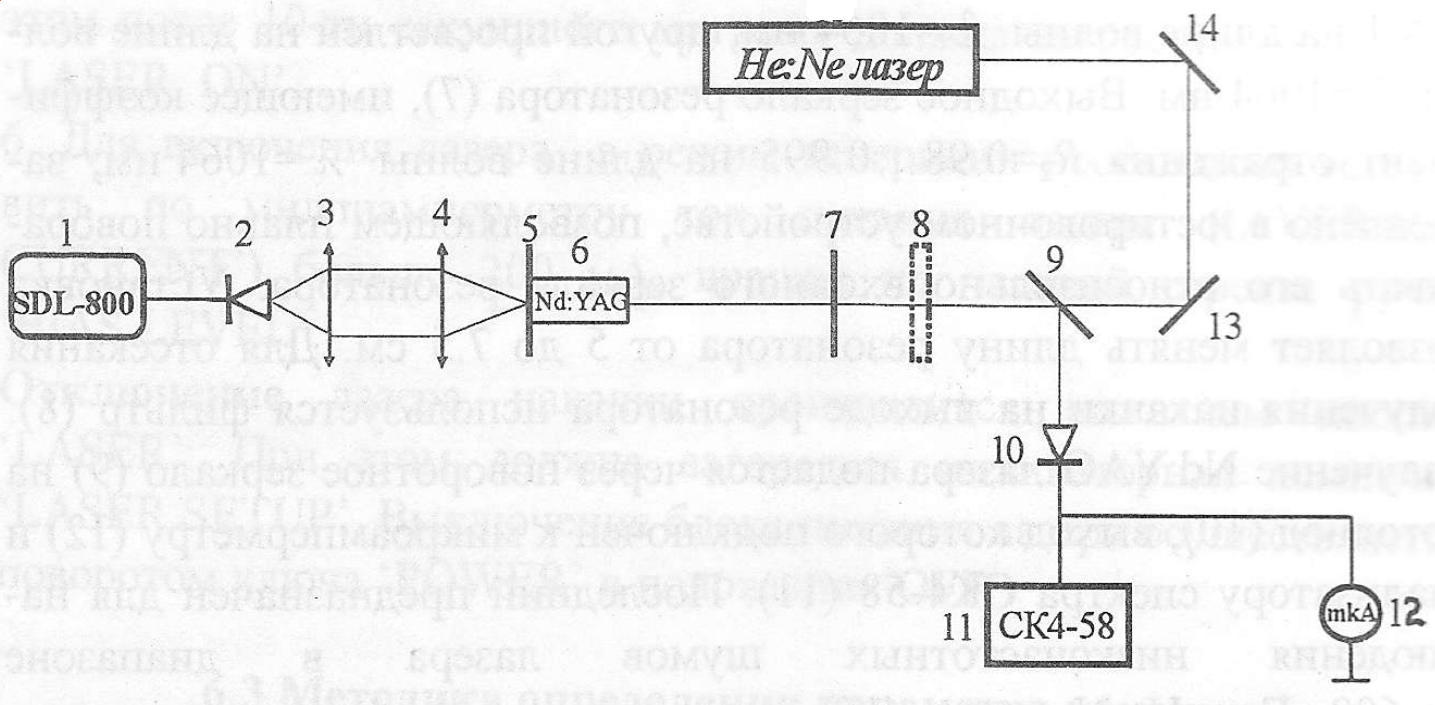
\includegraphics[width=\textwidth]{../figures/scheme.png}
		\caption{Схема установки.}
		\label{fig:scheme}
	\end{figure}

	Короткофокусная линза (3) используется для формирования параллельного пучка из сильно расходящегося у торца лазера излучения накачки. Линза (4) закреплена в поворотном устройстве, позволяющем перемещать луч накачки в горизонтальной и вертикальной плоскостях. Резонатор твердотельного лазера (5--7) установлен на платформе, передвигающейся в продольном и поперечном направлениях. В качестве активной среды лазера используется кристалл алюмоиттриевого граната YAG, легированный ионами $\mathrm{Nd}^{3+}$ с концентрацией 1\%. Кристалл Nd:YAG (6) имеет форму цилиндра длинной $1\,\text{см}$ и диаметром $0.6\,\text{см}$. Он закреплён в юстировочном устройстве, позволяющем плавно изменять положение оси кристалла относительно оси резонатора. Торцы кристалла имеют дихроичное покрытие. Один формирует входное зеркало резонатора (5), обеспечивая пропускание света $T\approx 1$ на длине волны $\lambda=810\,\text{нм}$ и отражение $R_1 \approx 1$ на длине волны $\lambda=1064\,\text{нм}$, другой просветлен на длине волны $\lambda=1064\,\text{нм}$. Выходное зеркало резонатора (7), имеющее коэффициент отражения $R_2=0.98\ldots0.995$ на длине волны $\lambda=1064\,\text{нм}$, закреплено в юстировочном устройстве, позволяющем плавно поворачивать его относительно входного зеркала резонатора. Установка позволяет менять длину резонатора от 5 до 7.5 см. Для отсекания излучения накачки на выходе резонатора используется фильтр (8). Излучение Nd:YAG лазера подается через поворотное зеркало (9) на фотодиод (10), выход которого подключен к микроамперметру (12) и анализатору спектра СК4-58 (11). Последний предназначен для наблюдения низкочастотных шумов лазера в диапазоне $0\ldots600$ кГц. He-Ne лазер (15) используется для юстировки резонатора. Для визуального наблюдения генерации Nd:YAG лазера используется карточка-визуализатор инфракрасного диапазона.

	\section{Протокол измерений}

	Измерили зависимость релаксационной частоты $f_\text{рел}$ и мощности излучения $P_\text{изл}$ от мощности накачки $P_\text{нак}$. Результаты измерений приведены в \tabref{tab}.

	\begin{table}[tb]
	\begin{center}
	 	\begin{tabular}{|c|c|}
	 		\hline
	 		$P_\text{нак}$, мВт & $f_\text{рел}$, кГц\\
	 		\hline
			216 &	112\\
			225 &	212\\
			235 &	276\\
			245 &	336\\
			255 &	392\\
			265 &	432\\
			270 &	448\\
			275 &	458\\
			280 &	476\\
			285 &	491\\
			296 &	508\\
			304 &	532\\
			345 &	551\\
			385 &	600\\
			390 &	616\\
			395 &	627\\
			405 &	639\\
			420 &	672\\
			\hline
	 	\end{tabular}
	 	\begin{tabular}{|c|c|}
	 		\hline
	 		$P_\text{нак}$, мВт & $P_\text{изл}$, мВт\\
	 		\hline
	 		420 &	9\\
			410 &	8.37\\
			400 &	7.85\\
			391 &	7.6\\
			381 &	7.3\\
			371 &	6.8\\
			361 &	6.1\\
			350 &	5.5\\
			340 &	4.6\\
			330 &	4\\
			320 &	3.76\\
			290 &	3.3\\
			280 &	2.9\\
			270 &	2.5\\
			260 &	2.1\\
			250 &	1.7\\
			239 &	1.2\\
			230 &	0.9\\
			220 &	0.5\\
			210 &	0.19\\
			200 &	0.14\\
			\hline
	 	\end{tabular}
	\end{center}
	\caption{Результаты измерений.}
	\label{tab}
	\end{table}

	\section{Результаты эксперимента с оценкой погрешности и их сравнение с теорией}

	\subsection{Определение пороговой мощности}

	Для дальнейшей работы важно определить пороговую мощность $P_\text{пор}$, ведь ниже будет часто использоваться параметр накачки $A$, который определяется как $P_\text{нак} / P_\text{пор}$ ($P_\text{нак}$ измеряется напрямую). Чтобы определить пороговую мощность $P_\text{пор}$, надо найти такую мощность накачки, что при мощностях накачки меньше данной мощность излучения равна нулю, а при больших мощностях накачки мощность излучения отлична от нуля.

	На \figref{fig:p_iz_vs_p_nak} показана снятая зависимость мощности излучения от мощности накачки с учётом фоновой засветки. Видно, что при $P_\text{нак}<210\,\text{мВт}$ излучения нет. Снятые данные дискретны и поэтому точно определить порог нам не удастся, мы лишь знаем, что при $P_\text{нак}=210\pm5\,\text{мВт}$ излучение есть, а при $P_\text{нак}=205\pm5\,\text{мВт}$ излучения нет. Порог находится где-то между $200\,\text{мВт}$ и $210\,\text{мВт}$. Значит, $P_\text{пор} = 205\pm5\,\text{мВт}.$

	% в теле документа
	\begin{figure} 
    	\centering
    	\begin{subfigure}[tb]{.49\textwidth}
			\centering
		 	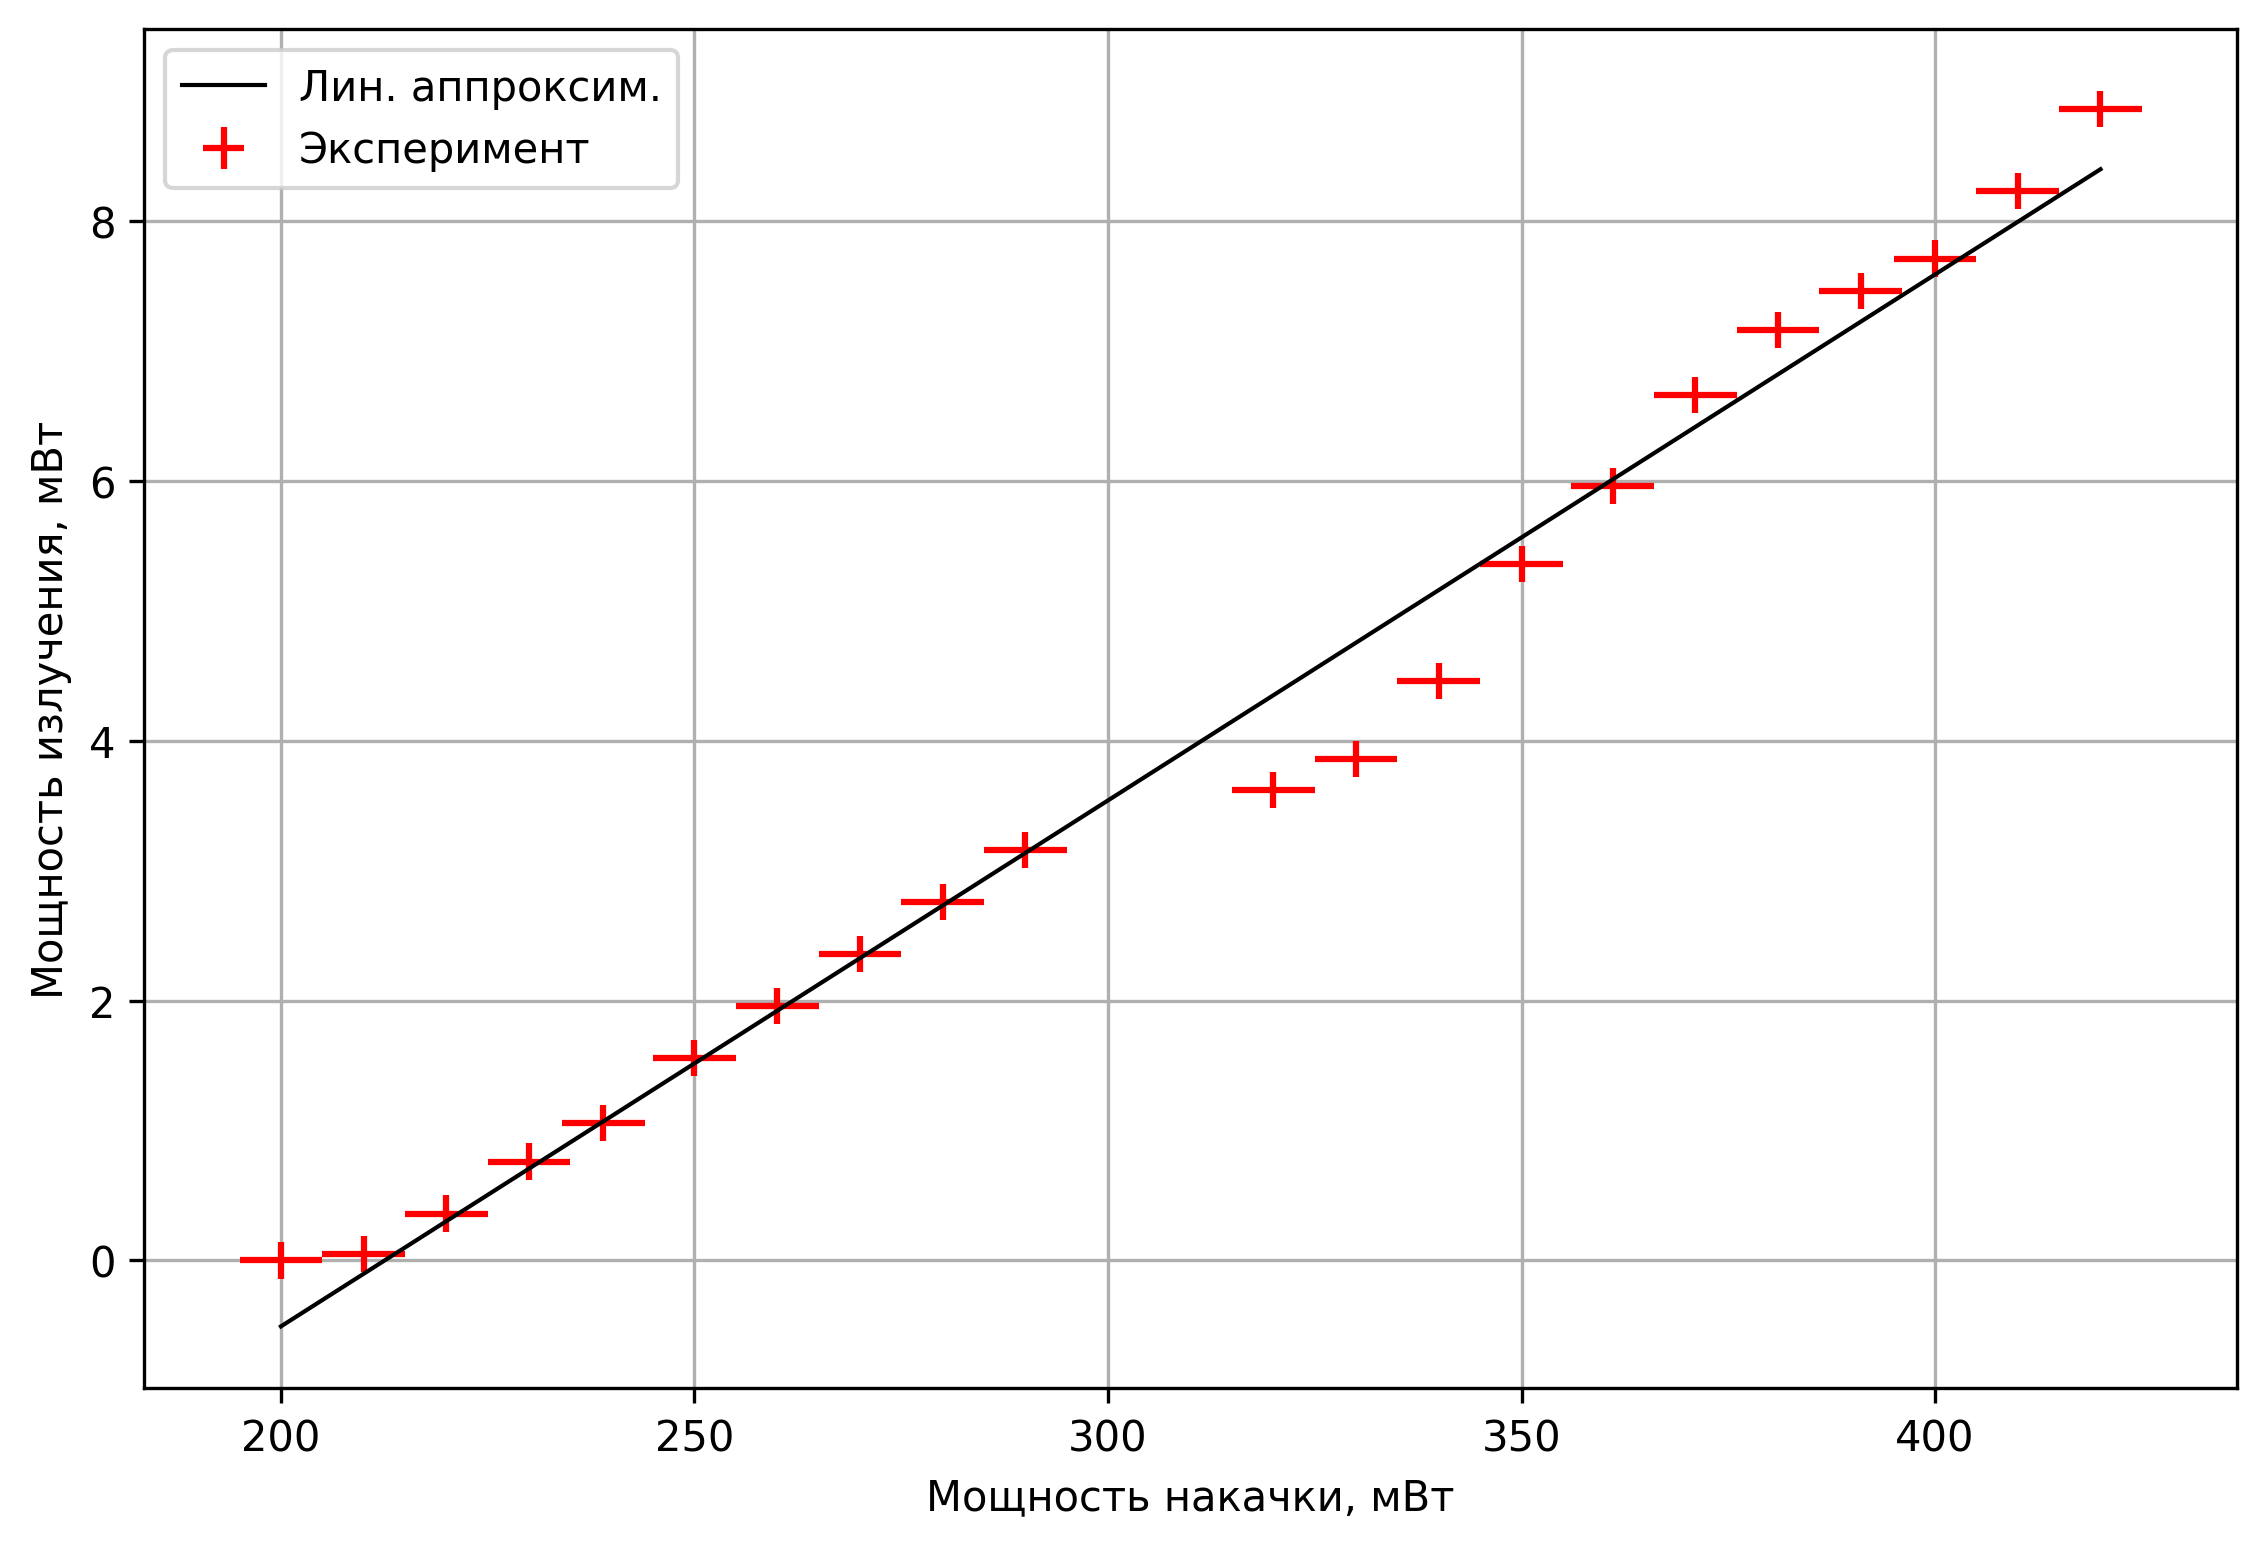
\includegraphics[width=\textwidth]{../figures/p_iz_vs_p_nak.png}
			\caption{}
			\label{fig:p_iz_vs_p_nak}
		\end{subfigure}
    	\hfill
    	\begin{subfigure}[tb]{.49\textwidth}
			\centering
			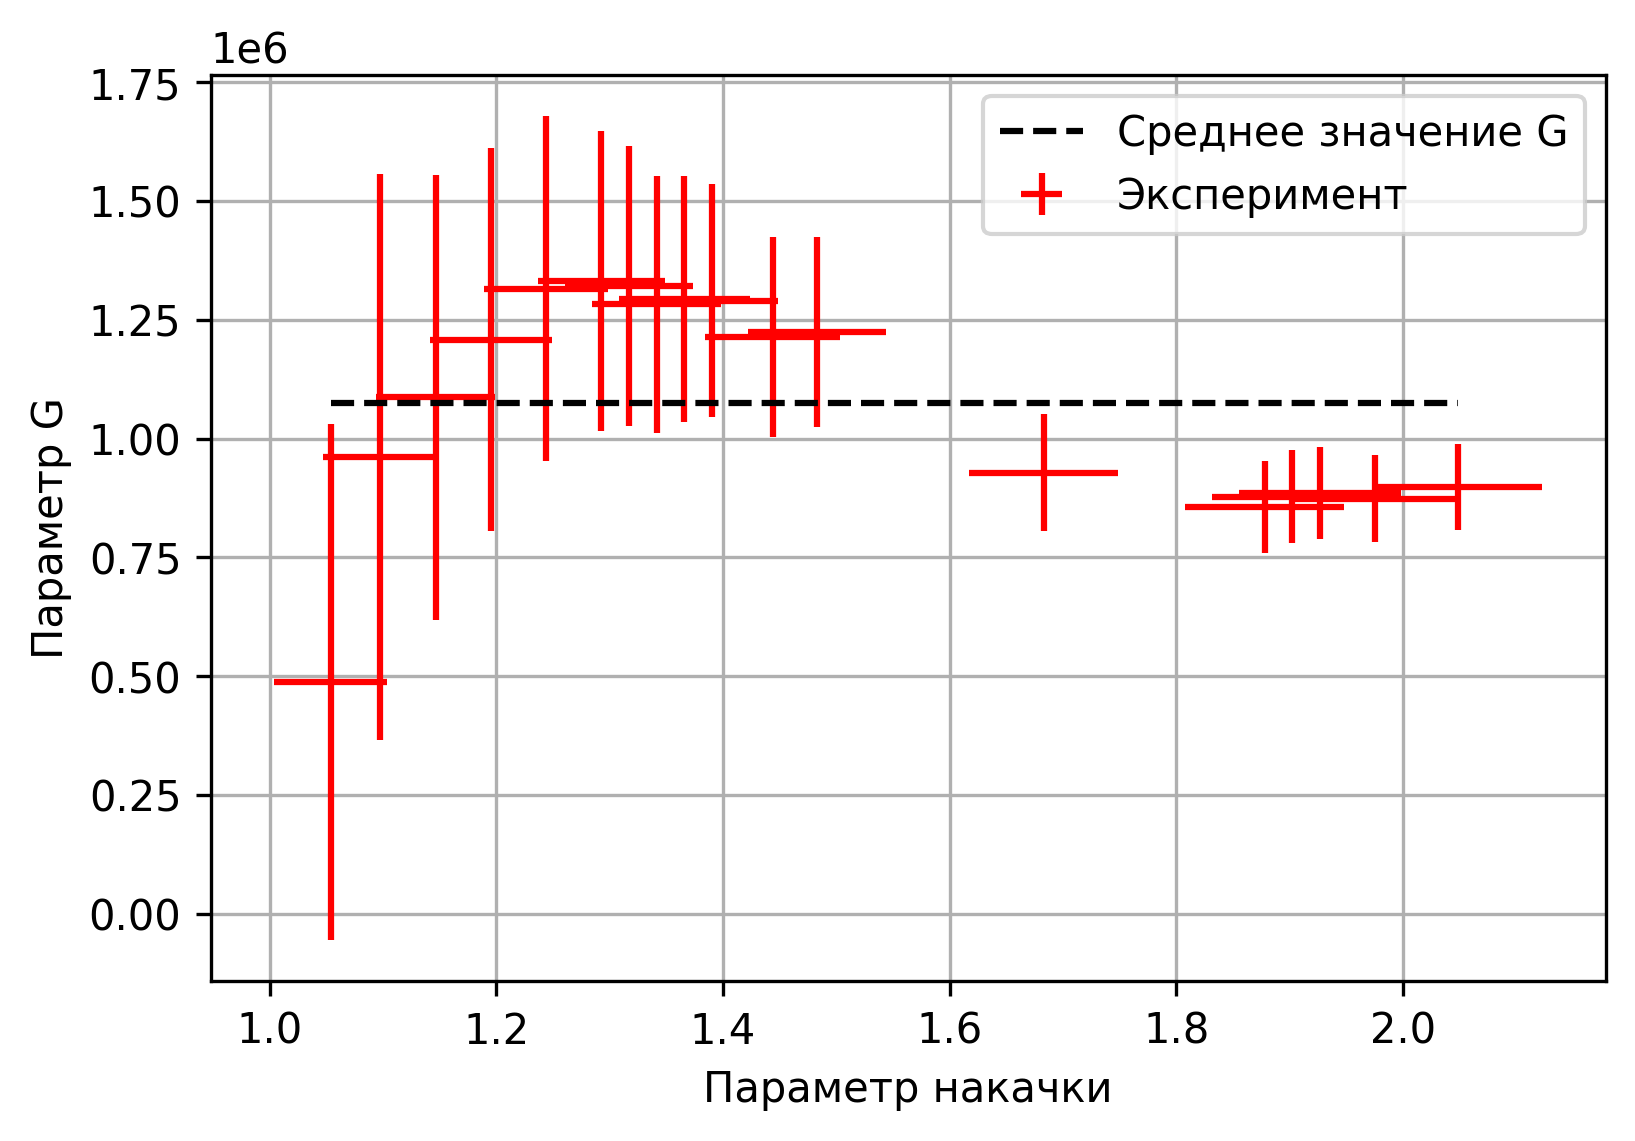
\includegraphics[width=\textwidth]{../figures/g_vs_a.png}
			\caption{}
			\label{fig:g_vs_a}
		\end{subfigure}
     	\caption{(a) Зависимость мощности излучения от мощности накачки. Фоновая засветка учтена и вычтена из мощности излучения. (b) Зависимость параметра $G$ от параметра накачки.}
	\end{figure}

	\subsection{Расчёт параметра G}

	Расчёт параметра $G$ проводился для каждого из экспериментальных значений параметра накачки $A$. Связь параметра накачки $A$ и параметра $G$ с измеренными значениями мощности накачки $P_\text{нак}$ и релаксационной частоты $f_\text{рел}$ даётся выражениями
	\begin{equation}
		A = \dfrac{P_\text{нак}}{P_\text{пор}},\quad \Omega = 2\pi f_\text{рел} T_1,\quad \Omega^2 = G\left( A - 1\right),
	\end{equation}
	где $T_1 = 0.23\,\text{мс}$ --- время релаксации насыщения.

	Конечная формула для $G$ и погрешности $\Delta G$
	\begin{equation}
	\begin{split}
		&G = \dfrac{\qty( 2\pi f_\text{рел} T_1 )^2}{A-1}, \quad \Delta_\text{изм}G = \dfrac{2(2 \pi T_1)^2 \, f_\text{рел}\, \Delta_\text{изм} f_\text{рел}}{A-1} + \dfrac{\qty( 2\pi f_\text{рел} T_1 )^2}{\qty(A-1)^2}\Delta_\text{изм} A,\\
		&\Delta_\text{изм} A = \dfrac{\Delta_\text{изм} P_\text{нак}}{P_\text{пор}} + P_\text{нак} \dfrac{\Delta_\text{изм} P_\text{пор}}{P_\text{пор}^2},
	\end{split}
	\end{equation}
	где $\Delta_\text{изм} f_\text{рел} = 10\,\text{кГц}$ --- измерительная погрешность измерения релаксационной частоты. % можно взять поменьше, наверно, но величина погрешности G всё равно будет оргомна

	На \figref{fig:g_vs_a} представлена зависимость параметра $G$ от параметра накачки $A$. Среднее значение $\langle G \rangle = 1.07\times10^{6}$. Найдём погрешность для параметра $G$
	\begin{equation}
		\Delta G = \sqrt{\qty(\Delta_\text{изм} G)^2 + \qty(\Delta_\text{случ}G)^2},
	\end{equation}
	где случайная погрешность считается как стандартное отклонение. Тогда можно записать для среднего значения параметра $G$
	\begin{equation}
		\langle G \rangle = \qty(1.07\pm0.35)\times10^{6}.
	\end{equation}

	\subsection{Графики зависимости мощности излучения и релаксационной частоты от параметра накачки}

	На \figref{fig:p_iz_vs_A} представлена зависимость мощности излучения $P_\text{изл}$ от параметра накачки $A$. Линейный тренд находился в виде $p\cdot(A - 1)$, где $p$ --- параметр, то есть линейный тренд проходит при $A=1$ через 0.

	

	На \figref{fig:Omega_vs_A} представлена зависимость мощности излучения $P_\text{изл}$ от параметра накачки $A$. Экспериментальные данные сопоставляются с результатами теоретическими, которые были построены по формуле $\Omega=\sqrt{\langle G \rangle (A-1)}$. Ошибки вычисления среднего значения $\langle G \rangle$ учтены синей областью на графике. Видно, что с учётом ошибок определения среднего значения $\langle G \rangle$ экспериментальные данные сходятся с теоретическими результатами.

	% в теле документа
	\begin{figure} 
    	\centering
    	\begin{subfigure}[t]{0.49\textwidth}
        	\centering
			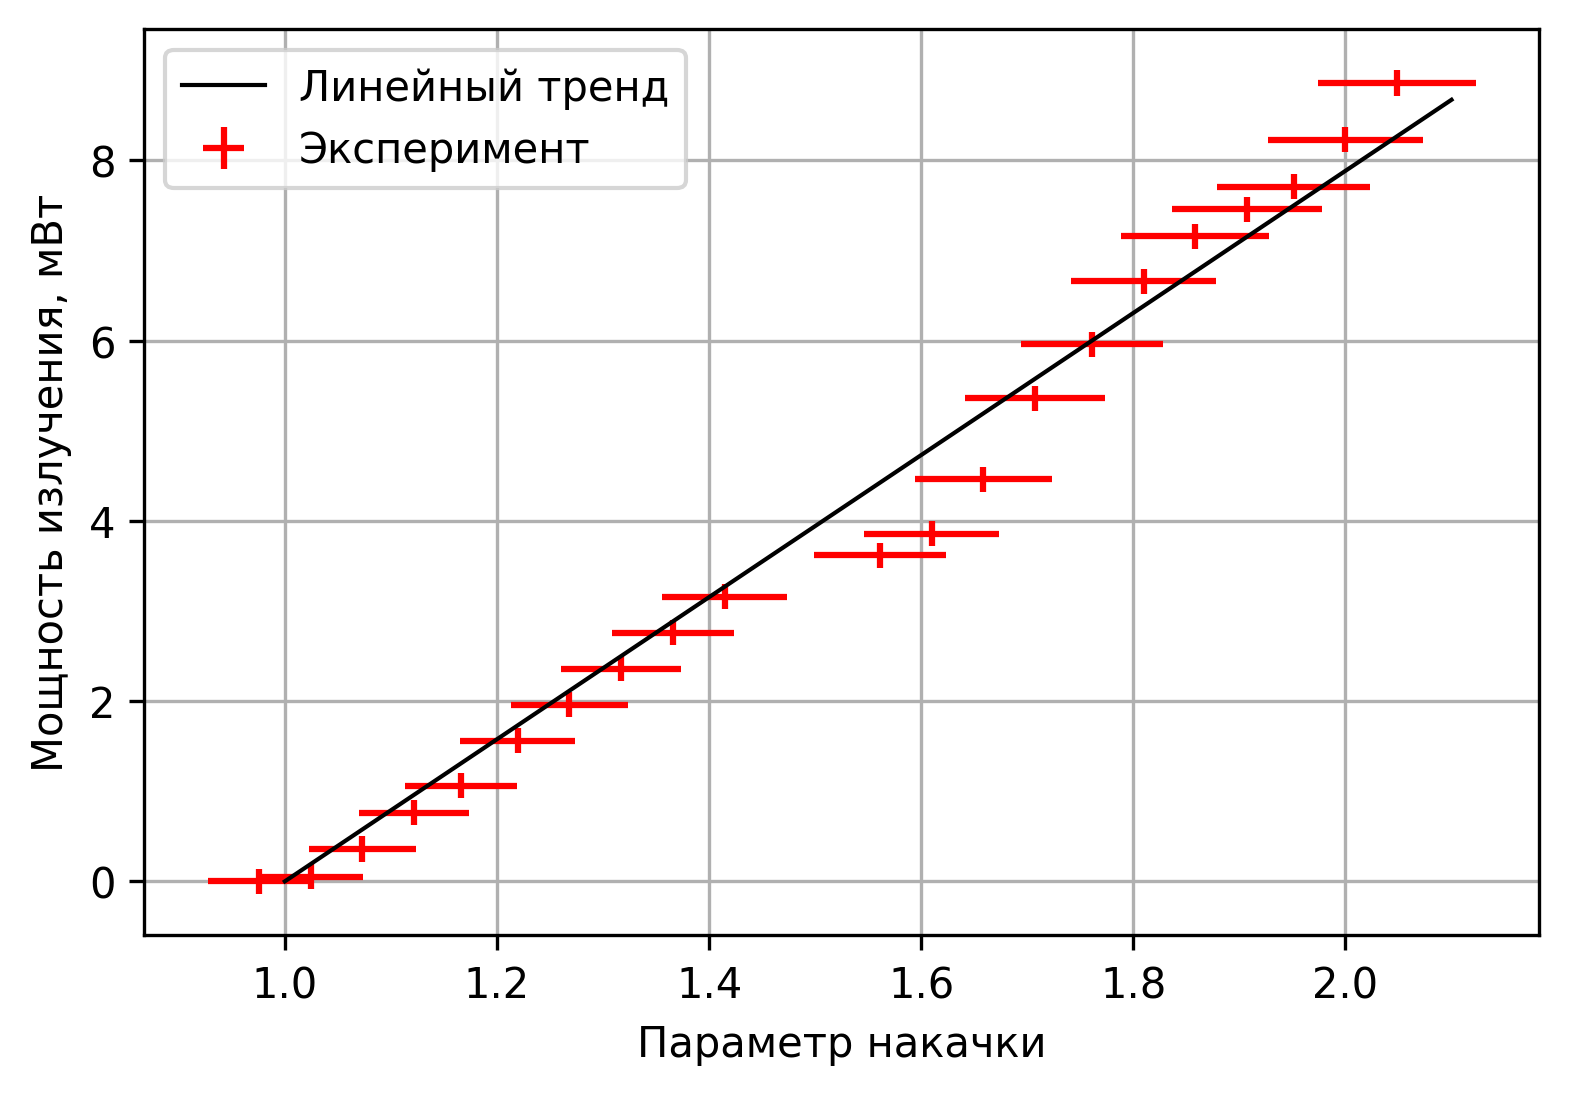
\includegraphics[width=\textwidth]{../figures/p_iz_vs_A.png}
			\caption{}
			\label{fig:p_iz_vs_A}
    	\end{subfigure}
    	\hfill
    	\begin{subfigure}[t]{0.49\textwidth}
        	\centering
			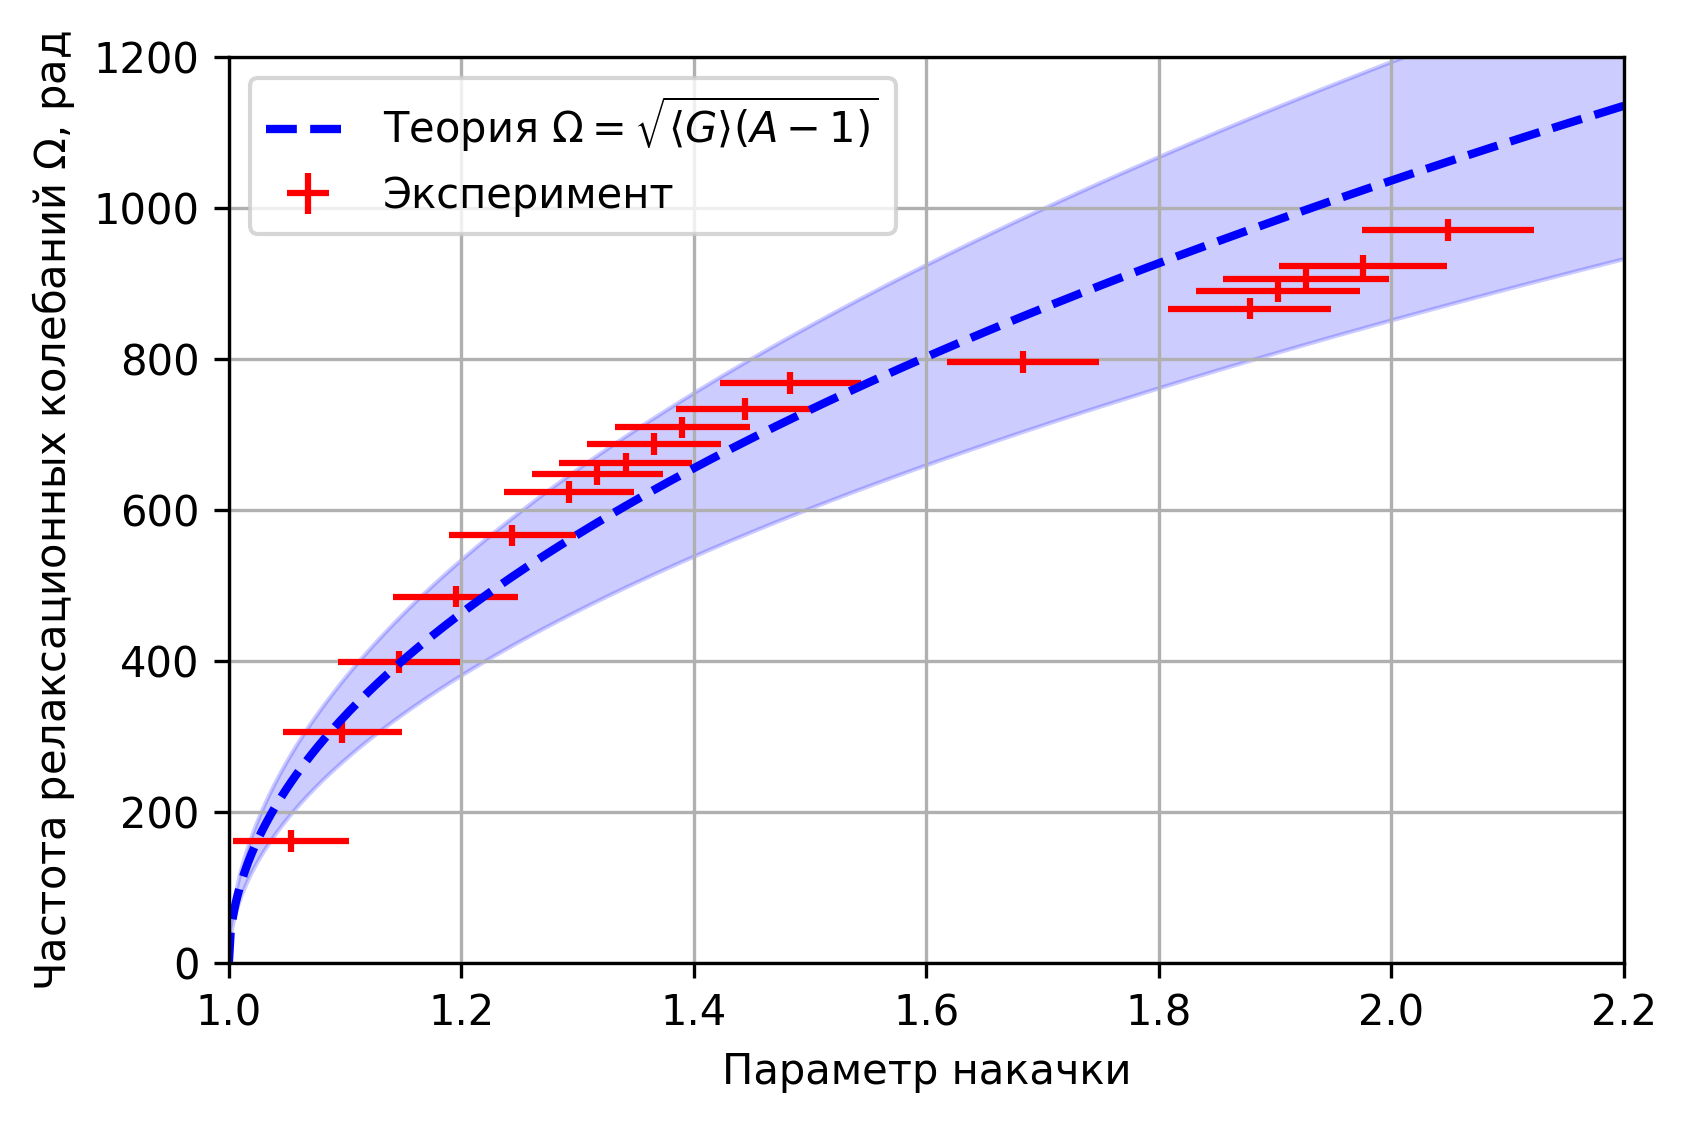
\includegraphics[width=\textwidth]{../figures/Omega_vs_A.png}
			\caption{}
			\label{fig:Omega_vs_A}
     	\end{subfigure}
     	\caption{(a) Зависимость мощности излучения $P_\text{изл}$ от параметра накачки $A$. (b) Зависимость частоты релаксационных колебаний $\Omega$ от параметра накачки $A$. Теоретическая кривая построена для среднего значения $\langle G \rangle$. Синяя область около теоретической кривой учитывает ошибку вычисления среднего значения $\langle G \rangle$.}
	\end{figure}

	\subsection{Оценка полосы резонатора лазера}

	Оценим по среднему значению $\langle G \rangle$ полосу резонатора лазера $\delta f_\text{эксп} = 1/(2\pi T_\text{с})$. По определению $G = T_1 / T_\text{с}$, тогда для $\delta f_\text{эксп}$ получаем выражение
	\begin{equation}
		\delta f_\text{эксп} = \frac{\langle G \rangle}{2\pi T_1}.
	\end{equation}
	Подставляем числа и с учетом погрешности получаем $\delta f_\text{эксп} = (7.44\pm2.43)\times10^8\,\text{Гц}$.

	\subsection{Сравнение оценочной величины полосы резонатора с теоретической}
	Теоретическое значение $$\delta f_\text{теор} = -\frac{c \ln{\sqrt{R_1 R_2}}}{2\pi L} \approx - 3\times10^8 \ln{\sqrt{1\times 0.98}}\; /\;(6.28 \times 0.01) = 4.83\times10^8\,\text{Гц}.$$ Взяли $L=1\,\text{мм}$. Теоретическое значение не совпадает в оценочной величиной даже с учётом погрешности. Стоит отметить, что если взять один из коэффициентов отражения хоть на одну сотую поменьше, то теоретическое значение будет совпадать с оценочным.

	\section{Природа многомодовости и отличие многомодовости для однородного и неоднородного уширения линий}

	Различают однородное и неоднородное уширение спектральных линий. При неоднородном уширении наблюдаемый профиль линии является суммой спектральных линий отдельных излучателей. Так, тепловое движение приводит к доплеровскому уширению спектральных линий (вследствие разброса скоростей отдельных атомов или молекул). Сдвиг длины волны отдельных излучателя в газовой или плазменной среде определяется проекцией его скорости на направление взгляда наблюдения.

	Однородное уширение спектральных линий связано с увеличением ширины энергетических уровней излучающей системы вследствие её зависящего от времени взаимодействия с возмущающим полем. Примером такого эффекта является ударное уширение спектральных линий, возникающее при столкновениях излучающей системы с электронами.

	Из формулы для $N_p$ (\ref{eq:N_p}) видно, что есть области пространства с нулевой инверсией внутри активной среды. Это так называемый эффект "выжигания" дырок. Дело в том, что в резонаторе Фабри-Перо поле моды имеет вид стоячей волны с периодом $\lambda_p/2$ и в узлах этой волны, где поле моды равно нулю, инверсия не уменьшается вследствие взаимодействия с полем. Разные продольные моды резонатора не совпадают, что служит причиной многомодовой генерации в лазерах с однородно уширенной линией усиления.

	При неоднородном уширении каждый отдельный излучатель среды излучает на своей длине волны, что приводит к многомодовой генерации в лазерах с неоднородным уширением спктральных линий.

\end{document}